\subsection{Reasoning transfer in CLEVR-CoGenT}
\label{sec:reasoning-transfer-clevr}
In the following experiments, we used CoGent-A only.
Using the question groups (categories) defined by the authors, we organized training and testing splits with the goal of measuring whether mastering reasoning for one questions group can help learning others.

\begin{figure}[htbp]
	\centering
	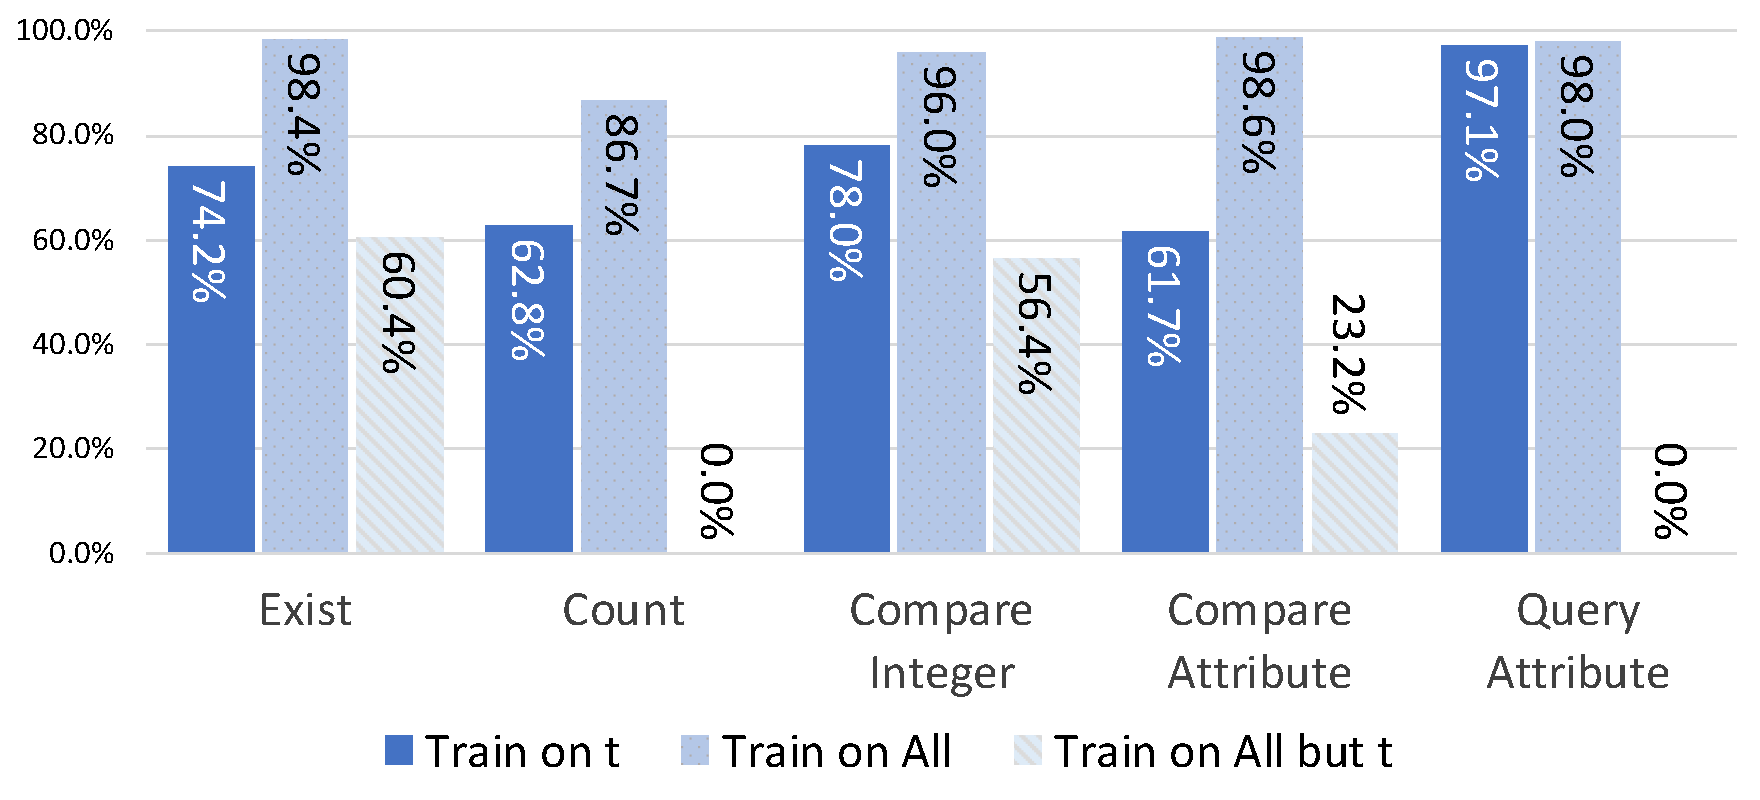
\includegraphics[width=\columnwidth]{../img/plots/cogent_reasoning_transfer.pdf}
	\caption{Accuracies of SAMNet when testing its reasoning transfer capabilities on the CoGenT-A variant.}
	\label{fig:cogent_reasoning_transfer}
\end{figure}

We first trained a single SAMNet instance and measured its accuracy on each of the task group $t$ separately.
Those results, indicated in \cref{fig:cogent_reasoning_transfer} as "Train on All", serve as baselines for the next two sets of experiments.

We next trained and tested 5 SAMNet instances, each on a single task group $t$ ("Train on t only").
We observe significant accuracy drops (from 18 up to almost 35 points) in all task groups, aside of \textit{Query Attribute}.
We hypothesize this results from the fact that mastering visual grounding and recognizing object attributes (being the core of the latter task) is a necessary skill the system needed by the other tasks.
Thus training on \textit{Query Attribute} helps others, whereas without any training on that particular group the system struggles with developing such a skill.

Finally, we trained 5 SAMNet instances in the extreme reasoning transfer setup: for each task group $t$ we trained a single instance on all tasks but $t$, and next tested its performance on $t$ only.
As expected, this setup appeared to be difficult to deal with, observing severe performance drops, with accuracy of \textit{Count} and \textit{QueryAttribute} dropping to zero.
The explanation is that these categories expect  answers (digits 0-9, names of attributes) that do not overlap with answers in the other groups (binary yes/no), thus the model cannot predict these labels on in a zero-shot transfer.

%Besides, the zero accuracy on \textit{Count} can also be explained by the fact that it results from the need of totally different reasoning leading to the answer.
%The \textit{QueryAttribute} latter is more interesting, as when mastering e.g.  \textit{Exist} of  \textit{CompareAttribute} the model \textit{had} to develop some kind of understanding object attributes.
%Still, this result once again suggests that the model learned joint representation of object attributes and struggle with disentangling them without being explicitly trained on task facilitationg that (like the  \textit{QueryAttribute}).



% An additional set of experiments, for which results are available in the supplementary material, fine-tune the model trained on all tasks on each task $t$ respectively.
%Fine-tuning did not demonstrate a clear benefit (except for \textit{Count}, where the accuracy increased by 1.5 pt) without hurting performance on the other tasks. Nevertheless, these experiments leave open the possibility that joint training of tasks may potentially benefit from using weighted sampling towards the tail end with more emphasis on samples from less performing task groups, similar to~\cite{guo2018dynamic, kendall2018multi}.

\subsection{Reasoning transfer in COG Canonical}
\label{sec:reasoning-transfer-cog}
In order to further investigate whether reasoning transfer was effective in leveraging information gained by training a task family at a higher level of the hierarchy we also conducted a setof  experiments using the Canonical variant of COG.
Order of the performed experiments is analogical to the one from previous section.
First column (\cref{fig:cog_reasoning_transfer}, "Train on All") is our baseline, i.e.
we train a single SAMNet instance on all tasks and test on each of the five task groups from the task hierarchy presented in \cref{fig:task-groups}.
Please note that those results are in fact weighted averages when aggregating accuracies of our model on the Canonical variant (\cref{fig:samnet_cog_detailed}).

\begin{figure}[htbp]
	\centering
	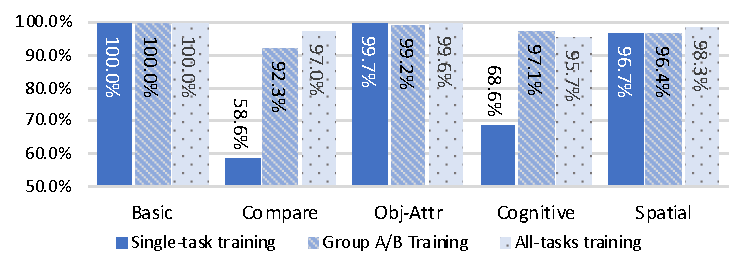
\includegraphics[width=\columnwidth]{../img/plots/cog_reasoning_transfer.pdf}
	\caption{Accuracies of SAMNet when testing its reasoning transfer capabilities on the Canonical variant of COG.}
	\label{fig:cog_reasoning_transfer}
\end{figure}

Next, we experimented with the "Train on t only" setup, i.e. training and testing each of 5 SAMNet instances on a single task group $t$ (i.e. single leaf of the proposed hierarchy).
For the \textit{Basic}, \textit{Spatial} and \textit{Obj-Attr} task groups the accuracy is matching the baseline, suggesting that each group contain tasks sufficient for developing all necessary skills.
Therefore models trained on those will not benefit from any additional training on other task groups.
However, the accuracy drops in the models trained only on tasks from the \textit{Compary} and \textit{Cognitive} task groups suggests the oposite.

For that reason we have performed the third set of experiments ("Train on Group A/B"), where we trained two SAMNet instances: first on tasks from the \textit{Group A} aggregate, tested next on each task from the lowest groups (i.e. \textit{Basic}, \textit{Obj-Attr} and \textit{Compare}) separately; and second on tasks from \textit{Group B}, tested separately on \textit{Spatial} and \textit{Cognitive}.
As expected, training on other tasks from group \textit{Group A} enabled the model to significantly improve on \textit{Compare} task (from 58.6\% to 92.3\%).
Similar improvement (from 68.8\% to 97.1\%) was observed in the second model, when trained on \textit{Group B} and tested on \textit{Cognitive}.
Moreover, the achieved accuracy is in fact higher by 1.4 point from the one achieved when training on all tasks (95.7\%).
This suggest that the model might have been struggling with mastering all that one when faced all kind of questions, maybe lacking the capacity.
Finally, there is an interesting effect for \textit{Obj-Attr} and \textit{Spatial}: training on the whole group A/B seems not to help the models, and when comparing those accuracies with the ones achieved by the models trained on task $t$ only we observe some slight drops (around 0.3-0.5 point).
Understanding that effect seems to require further investigation on dependencies between the resoning required by the particular questions and reasoning transfer.

%With \textbf{Spatial}, we see a small improvement showing that there is some benefit due to joint training with other task families.
%To further emphasize this behavior, notice that just joining \textbf{Compare} with \textbf{Obj-Attr} and \textbf{Basic} already causes a significant accuracy jump to 92.3\%.
%In hindsight, this is not surprising, as the questions in \textbf{Compare} are composed of fragments of questions given by \textbf{Basic} and \textbf{Obj-Attr}, and therefore can leverage the reasoning strategies developed there to reason about questions in \textbf{Compare}.
% Lastly, for the \textbf{Spatial} family, we again see the benefits of joint training with all questions (68.6\% to 95.7\%) but in this case there is a slight loss incurred by including everything. As seen in the figure, just jointly training with \textbf{Spatial} alone is sufficient to get a boost in accuracy (97.1\%). To summarize, while joint training helps, one needs to determine how much of correlation is present with the other tasks.
